\documentclass[12pt]{article}
\usepackage{graphicx}
\usepackage{fullpage}
\usepackage{amsmath,enumerate,here}
\usepackage{gensymb}


\begin{document}

\section{Part 1}

The total power $P$ delivered to the foil from the beam is given by the following equation where we assume a worst case scenario of a foil of thickness $\delta=25 \mu m$.

\begin{equation}
P=-\rho \frac{\mathrm{d} E}{\mathrm{d} x} \times N \times PRR \times \delta
\end{equation}

where $-\rho \frac{\mathrm{d} E}{\mathrm{d} x}$ is the energy loss of an electron per unit length of the foil, $N$ is the number of electrons in the bunch, and $PRR$ is the pulse repititon rate. Plugging in numbers for titanium gives the amount of power delivered over the small area of the foil.

\begin{equation}
P_{Ti}=7.17 \times 10^6 \frac{eV}{cm} \times 10^{10} \times 10 Hz \times 25 \times 10^{-4} cm \times \frac{1.6 \times 10^{-19} J}{1 eV}=0.0002868 W
\end{equation}

The amount of power per unit volume, assuming a beam size of $ \sigma = 25 \mu m$, is

\begin{equation}
S=\frac{P}{V}
\end{equation}

and for the titanium is

\begin{equation}
S_{Ti}=\frac{0.0002868 W}{\pi (20 \times 10^{-4})^2 \times 25 \times 10^{-4} cm^3}=9129 W/cm^3
\end{equation}

We will now compare the power input into the foil with the power radiated away due to temperature differences between the foil $T_1$ and the surroundings $T_2=300 K$.

\begin{equation}
q''_r=\epsilon \sigma (T_{1}^{4}-T_{2}^{4})
\end{equation}

where $\sigma$ is the Stefan-Boltzmann constant, $\epsilon$ is the emissivity of the foil, and $q''_r$ is the power emitted per unit area. For this analysis, we will assume that the foil is $50 \degree C$ below its melting point to obtain a worst case scenario. For titanium, this gives

\begin{equation}
q''_{r Ti}=0.2 \times 5.77 \times 10^{-12} (1900^{4}-300^{4})=15.03 W/cm^2
\end{equation}

And multiplying by the area gives

\begin{equation}
A=\pi \sigma^{2}=\pi (20 \times 10^{-4})^2=1.257 \times 10^{-5} cm^2
\end{equation}

\begin{equation}
P_{r Ti}=q''_{r Ti} \times A=0.000189 W
\end{equation}

Since the power radiated away is much less than the power deposited by the beam, most of the energy must be conducted away. We can start by searching for a steady-state solution to this problem assuming constant power being deilvered to the foil and no radiative heat loss. The difference in temperature between the foil $T_o$ and and the surroundings $T_i$ is given by

\begin{equation}
T_o-T_i=\frac{S \sigma^{2}}{4 K}
\end{equation}

where $k$ is the thermal conductivity of the foil. For titanium, this gives

\begin{equation}
(T_o-T_i)_{Ti}=\frac{9129 W/cm^3 (20 \times 10^{-4})^{2}}{4 \times 0.219 W/cm K}=0.0417 K
\end{equation}

Next, we can find the steady-state temperature difference $\Delta T$ (again assuming no radiative heat loss) between the spot where the beam deposits its energy and the remainder of the foil. We will also assume that the foil has a radius of $r_o=1.27 cm$. 

\begin{equation}
\Delta T=P' \frac{ln(\frac{r_o}{\sigma})}{2 \pi k}
\end{equation}

For titanium, this gives

\begin{equation}
\Delta T_{Ti}=\frac{0.0002868}{25 \times 10^{-6}} W/m \frac{ln(\frac{1.27 cm}{20 \times 10^{-4} cm})}{2 \pi 21.9 W/mk}=0.538 K
\end{equation}

Repeating the method for silicon after gives the following results

\begin{equation}
P_{Si}= 0.000155 W, q''_{r Si}=26.77 W/cm^2 , P_{r Si}=0.000337 W 
\end{equation}

\begin{equation}
(T_o-T_i)_{Si}=0.00334 K , \Delta T_{Si}=0.0430 K
\end{equation}

Now, in order to find the temperature profile as a function of $r$ and $t$, we use the heat equation for radial symmetry. We are assuming only conduction (without thermal radiation) in order to simplify the equation and to provide an upper bound.

\begin{equation}
\rho c_p \frac{\partial T}{\partial t}=\frac{1}{r} \frac{\partial}{\partial r} (k r \frac{\partial T}{\partial r})
\end{equation}

where $\rho$ is the density, $c_p$ is the specific heat, and $k$ is the thermal conductivity. The general solution to this equation is as follows.

\begin{equation}
T(r,t)=Ae^{-\alpha t} (c_1 J_0(\sqrt{\frac{\alpha \rho c_p}{k}}r)+c_2 Y_0(\sqrt{\frac{\alpha \rho c_p}{k}}r))
\end{equation}

where $J_0$ and $Y_0$ are Bessel function of the first and second kind, respectively, and $A$, $c_1$, and $c_2$ are arbitrary constants and $\alpha$ is related to how quickly the temperature decreases due to conduction. We must solve the equation for the following boundary conditions

\begin{equation}
T(0 \le r \le \sigma,0)=T_h, T(0,a)=T_0
\end{equation}

where $\sigma$ is the spot size of the beam, $T_h$ is the temperature immediately after the beam deposits energy into the foil, $a$ is the radius of the foil, and $T_0$ is the boundary temperature. This would be an interesting academic exercise.

\section{Thermal Radiation - Visible Photons}

In order to efficiently calculate the number of photons (or intensity) emitted due to a heated foil, we must make several assumptions. The most major assumption is that no conduction is present, i.e. the thermal radiation process is too quick for conduction to have effect. Second, the heated foil is only in a circle that is the same area as the cross-sectional area of the beam. Lastly, the foil heats to just below its melting point (50 $\degree$ in this calculation). These three assumptions are the "worst case scenario" and provide an upper bound to the problem. In this calculation, the relevant parameters used are the foil thickness ($\delta=25 \mu m$) and the beam size ($\sigma_r = 20 \mu m$). Calculations were carried out for both titaniu and silicon. We begin the calulation by relating energy $E$ to the temperature $T$ and the nominal temperature $T_0$.

\begin{equation}
E=V \rho c_p (T-T_0)
\end{equation}

where $\rho$ is the material density and $c_p$ is the specific heat of the material. Taking the time derivative gives the power $P$ in terms of the rate of change of temperature.

\begin{equation}
P=\frac{dE}{dt}=V \rho c_p \frac{dT}{dt}
\end{equation}

We also know that the total power given off by thermal radiation is simply the Stephen-Boltzmann Law.

\begin{equation}
P=-2 A \sigma \epsilon T^4
\end{equation}

where $A$ is the area of the heated portion of the foil, $\sigma$ is the Stephan-Boltzmann constant, and $\epsilon$ is the emissivity of the material. Since we are only considering radiation effects, we can set the equations equal to each other and obtain the following differential equation.

\begin{equation}
\frac{dT}{dt}=-\frac{2 A \sigma \epsilon}{V \rho c_p} (T^4-T_{0}^{4})=-\frac{2 \sigma \epsilon}{\delta \rho c_p} (T^4-T_{0}^{4})
\end{equation}

Notice that $\frac{A}{V}=\frac{A}{A \delta}=\frac{1}{\delta}$. Solving the differential equation is done simply by separation of variables, and integrating the temperature from the hottest temperature $T_h$ to $T$ and the time from $0$ to $t$ gives

\begin{equation}
ln(\frac{T-T_0}{T+T_0})-2tan^{-1}(\frac{T}{T_0})=-(At+C)
\end{equation}

where

\begin{equation}
A=\frac{8T_{0}^{3} \epsilon \sigma}{\delta \rho c_p}, C=ln(\frac{T_h+T_0}{T_h-T_0})+2tan^{-1}(\frac{T_h}{T_0})
\end{equation}

Unfortunately, we can only obtain an implicit function of $T$. However, since we only care about the case in which $T^4>>T_{0}^{4}$, the case where visible thermal radiation is dominant, we can neglect the $\sigma T_{0}^{4}$ term. This approximation is sufficient because of the 4th power temperature dependence, thus the differential equation reduces to the following.

\begin{equation}
\frac{dT}{dt}=-\frac{2 \sigma \epsilon}{\delta \rho c_p} T^4
\end{equation}

\begin{equation}
\int_{T_h}^{T} \frac{dT'}{T'^4}=\int_0^t -\frac{2 \epsilon \sigma}{\delta \rho c_p} dt'
\end{equation}

This yields the temperature as a function of time. The results for titanium and silicon are shown in the plot.

\begin{equation}
T(t)=T_h (1+\frac{6 \epsilon \sigma}{\delta \rho c_p} T_{h}^{3} t)^{-\frac{1}{3}}
\end{equation}

\begin{figure}
\begin{center}
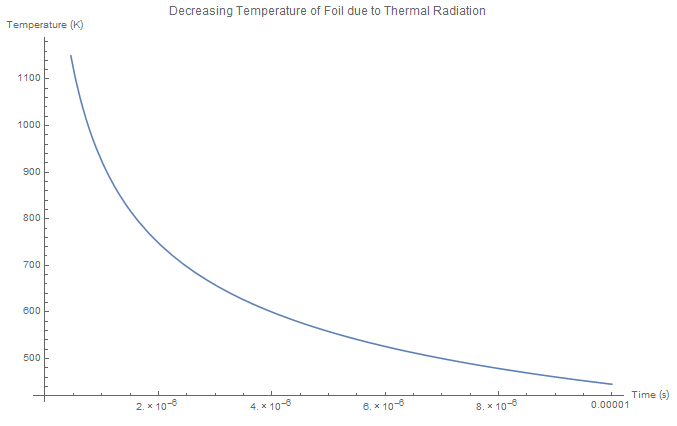
\includegraphics[scale=0.5]{figures/TemperatureTi.PDF}
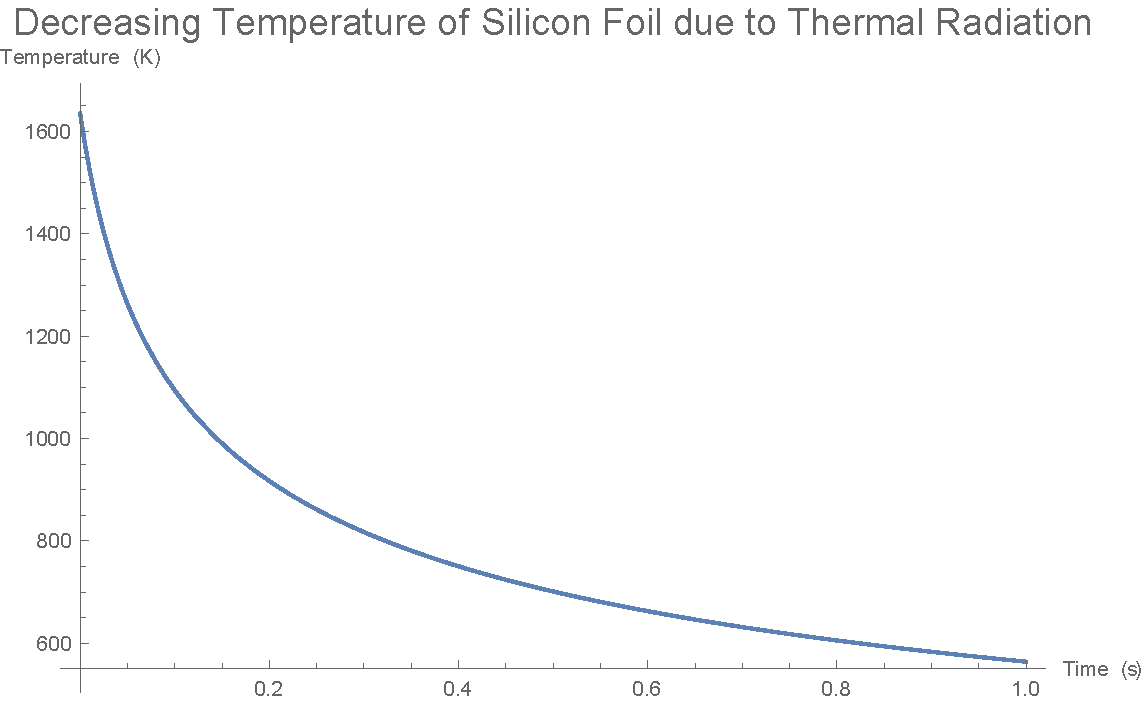
\includegraphics[scale=0.5]{figures/TemperatureSi.PDF}
\caption{This figure shows the temperature of the foil as a function of time for both titanium (a) and silicon (b). This neglects effects due to conduction.}
\end{center}
\end{figure}

In order to find the number of photons emitted, we start with blackbody radiation which gives the energy per area per solid angle per wavelength per time.

\begin{equation}
\frac{dE}{dA d \Omega dt d \lambda} = \frac{2 h c^2}{\lambda^{5}} \frac{1}{e^{\frac{hc}{\lambda k_B T}}-1}
\end{equation}

where $\Omega$ is the solid angle, $\lambda$ is the wavelength, $h$ is Planck's constant, $c$ is the speed of light, and $k_B$ is Boltzmann's constant. We can easily integrate over area ($A=\pi \sigma_r^2$) which is constant and the solid angle ($2 \pi$ since we are concerned with half of a sphere). In addition, we integrate over the visible spectrum (300 nm to 700 nm) and time to get the total energy due to visible photons as a function of time.

\begin{equation}
E(t)=4 \pi^2 \sigma_r^2 h c^2 \int_0^t \int_{\lambda_1}^{\lambda_2} \frac{1}{\lambda^{5}} \frac{1}{e^{\frac{hc}{\lambda k_B T(t')}}-1} d \lambda dt'
\end{equation}

In order to change energy to the number of photons, we used the simple quatized relationship and use the average wavelength $\lambda_{avg}$ as the wavelength.

\begin{equation}
E=n \frac{hc}{\lambda} \rightarrow n(t)=\frac{\lambda_{avg}}{hc} E(t)
\end{equation}

Plugging this equation into the above equation gives the total number of visible photons emitted due to thermal radiation as a function of time.

\begin{equation}
n(t)=4 \pi^2 \sigma_r^2 c \lambda_{avg} \int_0^t \int_{\lambda_1}^{\lambda_2} \frac{1}{\lambda^{5}} \frac{1}{e^{\frac{hc}{\lambda k_B T(t')}}-1} d \lambda dt'
\end{equation}

Taking the time derivative of the above equation (essentially removing the time integral) gives the rate of visible photons emitted due to thermal radiation as a function of time.

\begin{equation}
\frac{dn}{dt}(t)=4 \pi^2 \sigma_r^2 c \lambda_{avg} \int_{\lambda_1}^{\lambda_2} \frac{1}{\lambda^{5}} \frac{1}{e^{\frac{hc}{\lambda k_B T(t)}}-1} d \lambda
\end{equation}

The results for both titanium and silicon are shown in the following figures. From the figures, it is clear that the cooling time due to radiation is on the order of several seconds, after which it is important to take into account the radiation absorbed from the surroundings. During 0.1 s, the number of visible photons emitted from thermal radiation is approximately $8 \times 10^{11}$ for titanimum and $2 \times 10^{10}$ for silicon (divided by 2 because we only care about one side of the foil). This is actually comparable to the number of visible photons emitted due to transition radiation which is (for a 20 billion electron/positron bunch) about $3.39 \times 10^9$ for titanium and $0.856 \times 10^9$ for silicon. However, for the time that the camera detects photons, say about 10 $\mu s$, the number of thermal visible photons in that short period of time is about $1.1 \times 10^8$ for titanium and $1.8 \times 10^7$ for silicon. This is more than about a factor of 10 for titanium and 40 for silicon, even at worst case scenario (just below the melting point). In principle, one can compute the number of photons emitted due to thermal radiation during each camera shot by simply assuming a short time $t$, thus the photon rate and temperature will be approximately constant.

\begin{equation}
n(t) \approx 4 \pi^2 \sigma_r^2 c \lambda_{avg} \int_{\lambda_1}^{\lambda_2} \frac{1}{\lambda^{5}} \frac{1}{e^{\frac{hc}{\lambda k_B T}}-1} d \lambda \times t
\end{equation}



\begin{figure}
\begin{center}
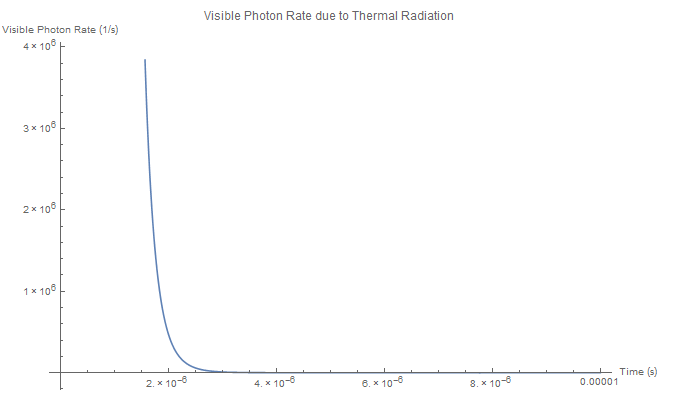
\includegraphics[scale=0.5]{figures/PhotonRateTi.PDF}
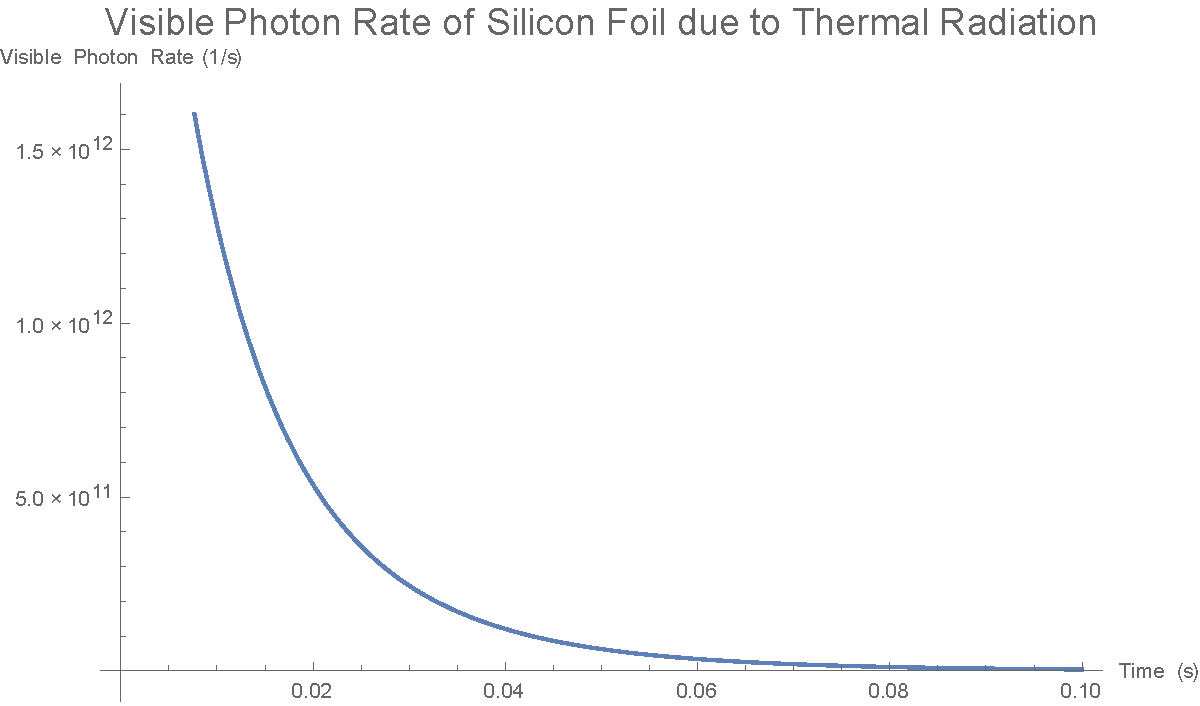
\includegraphics[scale=0.5]{figures/PhotonRateSi.PDF}
\caption{This figure shows the visible photon rate due to thermal radiation emitted from foil as a function of time for both titanium (a) and silicon (b). This neglects effects due to conduction.}
\end{center}
\end{figure}

\begin{figure}
\begin{center}
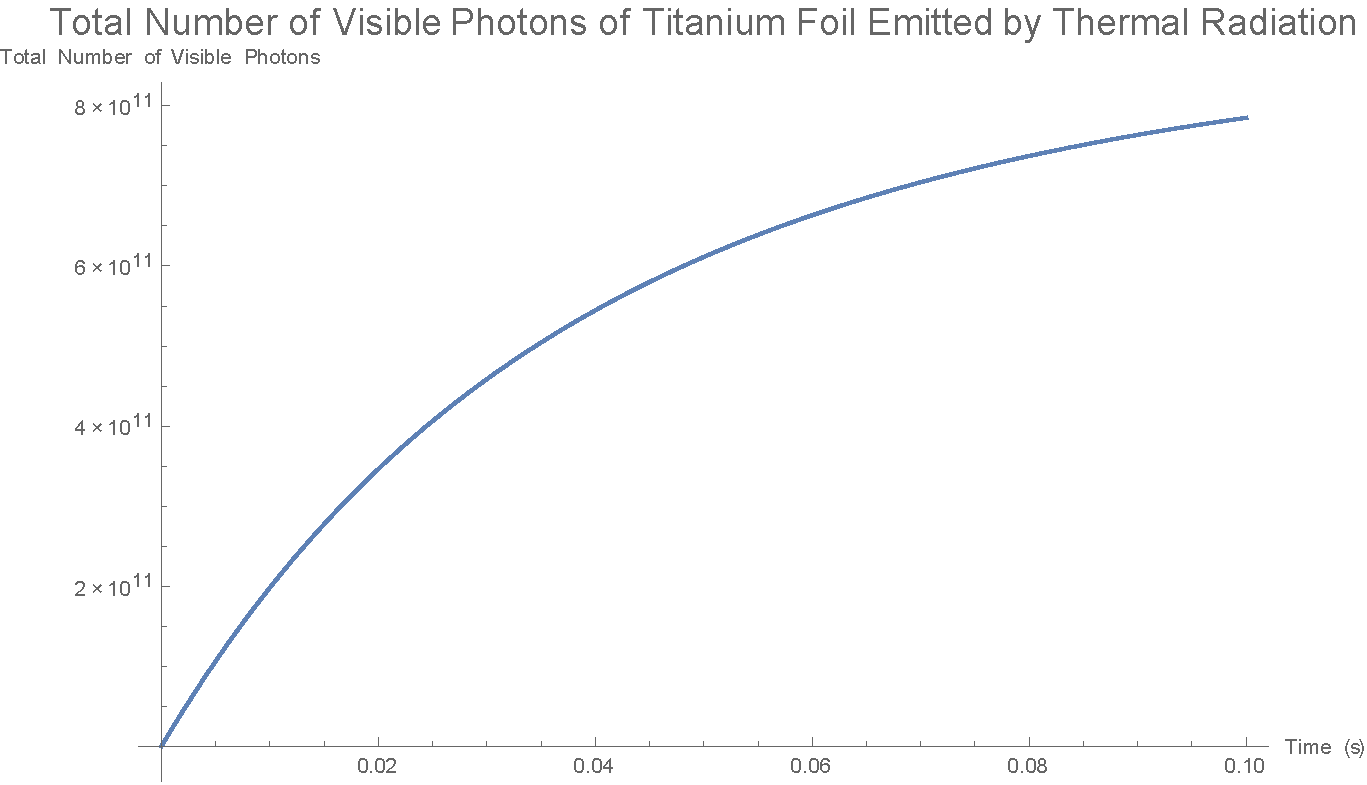
\includegraphics[scale=0.5]{figures/PhotonsTotalTi.PDF}
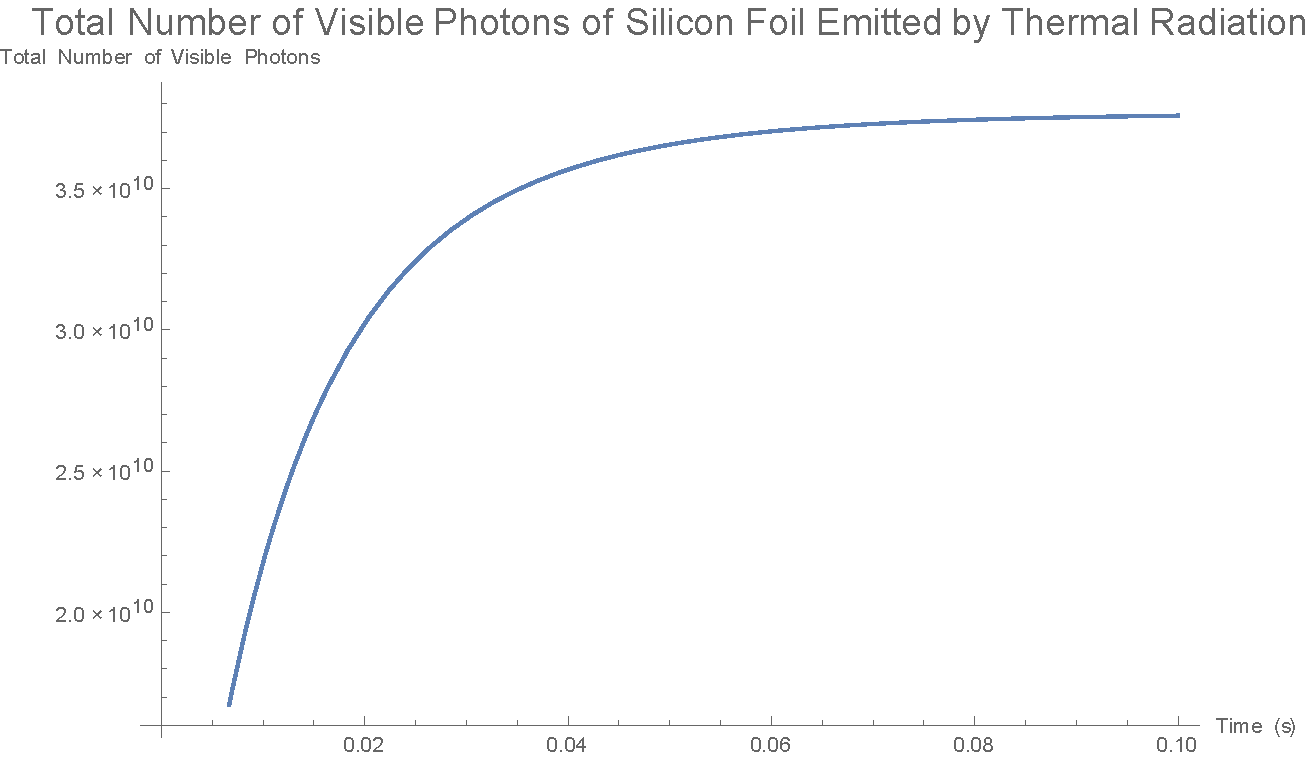
\includegraphics[scale=0.5]{figures/PhotonsTotalSi.PDF}
\caption{This figure shows the total number of visible photons emitted due to thermal radiation at time $t$ from the foil for both titanium (a) and silicon (b). This neglects effects due to conduction.}
\end{center}
\end{figure}

\end{document}